\section{Managing Trust}
\label{sec:mitigation}

The current trust situation inherent in using many cloud --
i.e. trusting many third parties with a wide range of capabilities and
only moderate disincentivizes to violating user trust -- is far from
ideal. This state places private user data and metadata at a high
degree of risk for unapproved exposure or manipulation. It is natural
to ask what solutions might aid in better controlling third party
trust arraignments, reducing the degree of risk involved when
leveraging third party services. While there are a myriad of potential
solutions in this space, ranging from technical to policy-based, I
suggest a few high level approaches to managing third party trust and
minimizing third party trust violations in this section.

The trust model presented in \S~\ref{sec:model} discusses two axis of
third party trust: the capabilities we entrust to third parties and
the manners in which this trust might be violated. Both axis can be
targeted when seeking to increase the security and privacy of user
data. By reducing the degree or trust -- i.e. limiting the number of
capabilities third parties are granted -- users can limit the amount
of harm a third party can inflict should this trust be violated. By
disincentivizing the various types of trust violations, a user can
decreased the likelihood that a third party violates their trust at
all. I'll discuss on strategies for pursuing both of these goals
below.

\subsection{Limiting Capabilities}
\label{sec:mitigation:capabilities}

Limiting the number of capabilities granted to third parties is an
obvious way to reduce the risk of privacy harms due to third party
trust violations. Furthermore, controlling which capabilities to
entrust to a third party is largely within the control of individual
end users, making this a relatively direct manner in which to reduce
the risk of harm from third trust violations. In the most extreme
case, users can simply elect to avoid using third party services,
effectively granting third parties no data-related capabilities at
all. For most users, however, such an approach is at best impractical,
and in some cases, simply not possible. Therein lies the crux of third
party capability reduction -- simply reducing capabilities is not
enough. Instead, users must have a way to both reduce capabilities
while also maintaining the ability to benefit from third party
services in the manners to which theory are accustomed. Thus, the true
aim of third party trust reduction is to identify ``trust surpluses''
-- situations where third parties are being trusted with more
capabilities than are strictly necessary to provide the benefits the
user derives from the service. Finding and eliminating such surpluses
allows users to reduce the degree by which they must trust third
parties while also continuing to leverage third party services to
provide desirable benefits.

Fortunately (at least from the perspective of users hoping to find
ways to reduce the amount they must trust third parties), trust
surpluses appear to be relatively common in modern third party
services. Take, for example, the Dropbox file syncing service. As
discussed in \S~\ref{sec:analysis:capabilities}, users must currently
entrust Dropbox with all available capabilities: storage (\emph{S}),
access (\emph{R}), modification (\emph{W}), and metadata
(\emph{M}). In order to provide Dropbox's core service, however,
Dropbox only requires a single capability: storage. Thus, granting
Dropbox the access, modification, and metadata capabilities represent
a trust surplus that can conceivably be eliminated without reducing
Dropbox's ability to provide the syncing and sharing benefits users
expect.\footnote{The techniques discussed herein focus primarily on
  limiting surplus access and manipulation
  capabilities. Unfortunately, limiting the metadata capability is
  historically much more difficult than limiting capabilities such as
  access or manipulation. Thus, until better solutions present
  themselves, it may be necessary to continue granting third party
  service providers the metadata capability -- even in surplus.}

The question then becomes how best to limit Dropbox's access to these
surplus capabilities. As mentioned previously, client-side
cryptographic techniques provide tools for liming the access
capability (e.g. encryption) as well as the modification capability
(e.g. authentication). In the case of Dropbox, a client could encrypt
and authenticate their data prior to uploading it to Dropbox and then
decrypt and verify the data when retrieving it from Dropbox. Dropbox
is unable to read or modify such encrypted and authenticated data when
stored on their servers. Such techniques, however, have a
downside. Namely, they require the user to mange and maintain certain
secrets to which Dropbox is not privy -- namely the private keys
necessary to perform data encryption or authentication. Furthermore,
the user must find a way to manually distribute these keys across any
device from which they wish to access their Dropbox files, or share
them with any user with which they wish to share their Dropbox
files. These requirements impose an additional burden on the user,
violating the original premise that users should be able to reduce
third party trust without also reducing their ability to derive
benefits from third party services. Such burdens significantly reduce
the ease of use that draws so many users to solutions such as Dropbox.

There are mechanisms, however, that allow users to both leverage
cryptographic techniques to limit Dropbox's capabilities while also
avoiding the need to impose additional usability burdens on users. For
example, the user could turn to an additional third party Secret
Storage as a Service (SSaaS) service capable of automatically storing,
syncing, and sharing user secrets such as cryptographic keys on the
user behalf. Such a service is discussed in depth
at~\cite{custos-trios}. When used in conjunction with a traditional
cloud storage provider such as Dropbox and existing cryptographic
techniques, a secret storage service can be employed to transparently
limit third party trust without imposing any additional burden on the
end user~\cite{sayler-phd}. In such an arrangement, the end user
stores only encrypted and authenticated file data with Dropbox,
limiting Dropbox's access to the \emph{R} and \emph{W}
capabilities. The user than stores the associated cryptographic
secrets with a secret store provider (SSP) capable of controlling
access to the secrets in a user defined manner and syncing or sharing
them as requested. Neither Dropbox (called a ``feature Provider'' (FP)
in the SSaaS model due to the fact that they primary exist to provide
an end-user with a feature-focused service) nor the SSP have the
ability to access or manipulate user data since Dropbox lacks the keys
necessary to perform such operations and the SSP lacks the data on
which these operations are to be performed.
Figure~\ref{fig:mitigation:trust} illustrates such an
arrangement. Thus, the user has successfully eliminated two of the
surplus capabilities traditionally granted to Dropbox in a manner that
allows them to continue using Dropbox to sync and share files as they
are accustom.

\begin{figure}[t]
  \centering
  \begin{subfigure}[t]{0.48\textwidth}
    \centering
    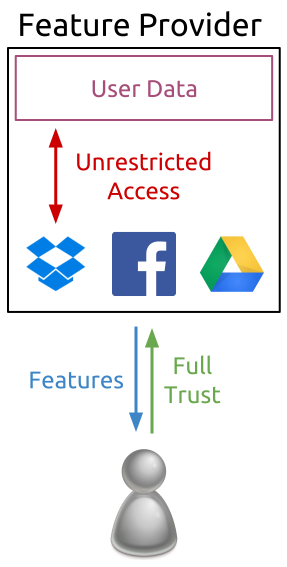
\includegraphics[height=2in]{./figs/out/TrustModel-Traditional.pdf}
    \caption{Traditional Trust Relationship}
    \label{fig:mitigation:trust:traditional}
  \end{subfigure}
  ~
  \begin{subfigure}[t]{0.48\textwidth}
    \centering
    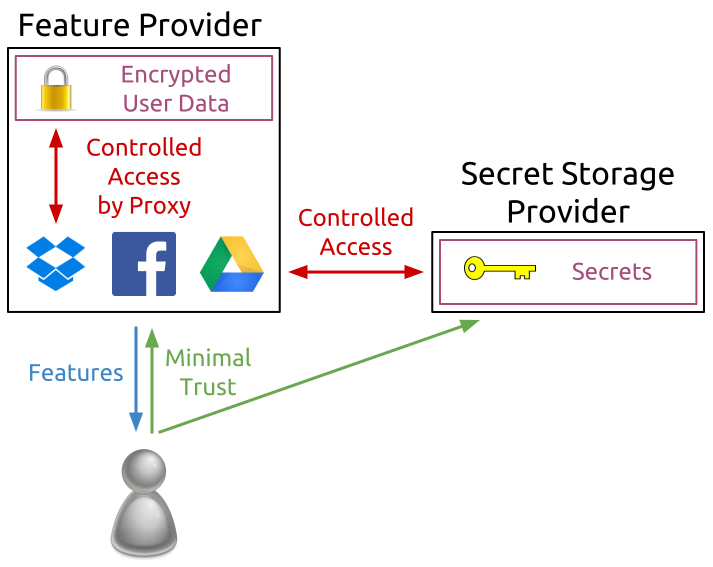
\includegraphics[height=2in]{./figs/out/TrustModel-Seperated.pdf}
    \caption{Distributed Trust Relationship}
    \label{fig:mitigation:trust:distributed}
  \end{subfigure}
  \caption{SSaaS Model Relationships}
  \label{fig:mitigation:trust}
\end{figure}

Techniques such as these are a from of ``trust distribution'' --
e.g. a technique for reducing trust in individual third parties by
instead spreading it across multiple parties. Similar techniques have
been used within cryptographic protocols for the purpose of
eliminating single-points-of-trust~\cite{shamir1979}.\footnote{Such
  techniques also bear some resemble to previously proposed ``key
  escrow systems'', albeit with a somewhat opposite
  end-goal~\cite{denning1996}: escrow systems aim to allow additional
  third parties access to user data whereas trust distribution systems
  aim to reduce the access to user data any single party can achieve.}
Trust distribution techniques are capable of allowing users to reduce
or eliminate trust surpluses across a range of use cases without
introducing significant additional usage burdens. While there are
approaches to limiting third party trust that aim to avoid trusting
any third party (e.g. the OTR chat protocol~\cite{otr-v3}), such
techniques are often difficult to apply generally or to use without
imposing additional usability burdens on end users. Trust distribution
strategies, however, provide a relatively generic framework for
eliminating trust in any single third party.\footnote{When coupled
  with techniques such as~\cite{shamir1979}, trust reduction
  techniques can eliminate trust in even larger subsets of all
  involved parties, e.g. not having to trust up to three of any five
  parties.}

To summarize, the proposed recipe of reducing the number of trusted
capabilities afforded to third parties is as follows:

\begin{packed_enum}
\item Identity any surplus trusted capabilities
\item Leverage cryptographic techniques to limit third party access to
  these capabilities
\item Leverage trust distribution techniques such as SSaaS to store
  and control access to any secret materials required by the
  aforementioned cryptographic techniques in a manner that avoids
  burdening the end user with the need to manage such secrets
  manually.
\end{packed_enum}

This process eliminates trust surpluses by distributing user trust
across multiple third parties in a manner such that individual third
parties can not subvert this trust. As mentioned in
\S~\ref{sec:analysis:violations}, such arrangements do have the
potential to encourage collusion-type trust violations where multiple
third parties work together to regain capabilities that have bean
denied to them. Mechanisms for disincentivizing such violations will
be discussed in the next section.

\subsection{Disincentivizing Violations}
\label{sec:mitigation:violations}

Beyond limiting the number of capabilities users must entrust to third
parties, it is also desirable to disincentive the mechanisms by which
third parties might violate such trust.  While technological solutions
provide options for reducing degree of trust, it is largely policy
solution that will drive the disincentivization of common classes of
trust violations. By disincentivizing certain classes of trust
violations, we can reduce the likelihood that third parties will
commit such violations, leading to more ``trustworthy'' third parties
and fewer instances of trust violations. There are a variety of
mechanism that one might employ with an aim toward disincentivizing
trust violations. I discusses several of the more prominent ones in
this section.

\subsubsection{Distributed Trust Markets}

In today's traditional third party trust relationships, users
primarily select third party services on the basis of their
features. When users pay for these services, they're primarily paying
to support the core features such services provide. Privacy and
security, while potential end-user concerns, are at best secondary
goals. Furthermore, on many free cloud services, the ability to
harvest user data is the basis of the service provider's business
model. As discussed in Section~\ref{sec:mitigation:capabilities}, these
situations create a number of perverse incentives in terms of a third
party's respect to user security and privacy. In the first case, the
third party simply does not prioritize user security since that is not
the primary basis on which users are choosing to use a service. In the
second case, a third party service provider actively works to subvert
user privacy in order to further leverage user data to generate
income.

Distributed trust relationships (Figure~\ref{fig:mitigation:trust}),
such as those employed by the aforementioned SSaaS model, aim to
rectify these issues by introducing additional third party actors
whose primary goal is the protection of user secrets and by proxy, the
data such secrets can be used to cryptographically protect. The
ability of distributed trust architectures to separate
privacy-oriented secret storage duties from feature-oriented service
provider duties allows users to purchase each service on the basis of
its associated merits. This quality avoids the issues associated with
putting desirable features in direct competition with security and
privacy -- a competition that security and privacy have historically
lost. Thus, distributed trust relationships not only allow users to
eliminate trust surpluses as discussed in
\S~\ref{sec:mitigation:capabilities}, they also allow users to escape
from traditional, but largely artificial, trade offs between desirable
third party features and the control of their data. Given such
separation, independent markets can form around feature provision and
secret protection, optimized for the respective priorities of each
field.

In order to achieve such a market, it is necessary to standardize on a
single distributed trust protocol. Such a standard protocol gives
users a high degree of mobility between competing secret storage
providers, avoiding vendor lock-in. This mobility, in turn, increases
the competitive pressures between providers. In short, the aim of a
distributed trust ecosystem is to make security and privacy tradable
commodities, and to leverage market powers to price and improve
both. A competitive market for secret storage has a number of security
and privacy enhancing benefits:

\begin{packed_desc}
\item[Reputation:] If users can easily switch between secret storage
  providers, it forces such providers to compete on the basis of their
  security and privacy preserving reputations. Providers who can do a
  superior job avoiding the trust violations discussed in
  \S~\ref{sec:analysis:violations} can attract more users and/or
  command a higher price for their services. Since a secret storage
  provider reputation is tied solely to their ability to faithfully
  protect user secrets, they will not be able to ``iron over'' any
  privacy-related reputation failings with superior end user feature
  sets -- a practice employed by many traditional feature
  providers.\footnote{As an example, consider Facebook's numerous
    trust violations~\cite{goel2014, lomas2014, tsukayama2014} and the
    fact that such violations have had no noticeable impact on the
    number of people using Facebook~\cite{foster2014}. A secret
    storage provider would enjoy no such network benefit from
    providing additional services beyond secret storage were they to
    violate user's trust; instead, users would simply switch to a new
    provider.}
\item[Multiple Providers:] A healthy ecosystem of competing secret
  storage providers will allow users to select from multiple
  independent providers over which they may further distribute their
  trust beyond a binary feature provider + secret storage provider
  relationship. Such sharding provides a number of benefits over
  relying on a single SSP, from additional trust reduction to data
  redundancy.
\item[Cost:] As in other competitive markets, having a number of
  competing providers will allow the user to select a provider that
  offers the best combination of cost and service.
\end{packed_desc}

Distributed trust markets are potentially useful at disincentivizing a
range of trust violations, from implicit violations to unintentional
violations. Such markets help to align economic incentives with
practices that disfavor such violations.

\subsubsection{Digital Due Process}

While mechanisms such as distributed trust markets are useful for
disincentivizing many classes of trust violations, other mechanisms
are needed to disincentive compelled violations. Trust markets
potentially encourage third parties to push back against compelled
trust violations to the maximum extent permitted under the law, but
they do little to protect users in cases where the law requires such
violations. While there are some cases where such violations are in
the public interest, it appears that in many (if not most) compelled
violations cases, the public interest in not being well
served~\cite{greenwald-prism, greenwald-collect}. To reduce such
unnecessary compelled violations, it is important to ensure ``digital
due process'' rights.

The first step toward protecting such rights is to ensure that user
data stored or processed by third party services receives the same
level of protection as data stored or processed locally. This concept
runs counter to the Third Party Doctrine established by current
U.S. case law~\cite{thompson-thirdparty}. This doctrine holds that
individuals who voluntarily store their data with third parties have
no ``reasonable expectation of privacy''~\cite{scotus-katzvus} for
such data. While such a viewpoint may have made sense in the
mid-20\textsuperscript{th} century when it was established via a
series of Supreme Court rulings~\cite{scotus-usvmiller-privacy,
  scotus-smithvmaryland}, it does not translate well to a world where
third party access to user data is the norm. As shown in
\S~\ref{sec:analysis:violations} compelled violations are a growing
trend, and in many cases, such violations are served via third-party
doctrine mechanisms. Such trends suggest a likely overreach of
government data collection, leading to a range of adverse ``chilling''
effects (e.g.~\cite{penney2016}). One possible way of halting or
reversing this trend would be to eliminate the third party doctrine
and begin requiring a 4\textsuperscript{th} Amendment warrants in
order to compel third parties to provide or modify user data.

Fortunately, changes to the third party doctrine are beginning to
progress on multiple fronts. Recent Supreme Court decisions have
suggested a willingness to expand user privacy rights in the digital
realm, and may eventually lead the Supreme Court to revisit the third
party doctrine~\cite{scotus-usvjones}.  Congress has also long been
debating updates to third-party doctrine derived laws such the
Electronic Communications Privacy Act (ECPA)~\cite{ecpa} to include a
warrant requirement for digitally stored
emails~\cite{eff-ecpareform}. Recently, the U.S. House of Represents
unanimously passed a bill to amend the ECPA to required warrants in
most cases~\cite{trujillo-ecpa}. Such movements suggest a growing
recognition of the due process rights of digital data, regardless of
whether it is stored locally or by third parties. Such trends likely
represent the best hope for reducing unnecessary compelled violations,
ensuring such violations only occur in cases where the public interest
in significantly favored by the compelled violation of user trust.

\subsubsection{Third Party Liability}

Another mechanism for disincentivizing trust violations, especially of
the unintentional variety, would be to establish standards of
liability for trust violations that result in harms to user
privacy. If a third party violates a users trust, and harms the user
in the process, it is reasonable to expect that users should be able
to seek some measure of relief for such violations. Trust violation
liability would follow the growing trend toward holding companies
liable for digital data breaches resulting from poor security
practices (e.g.~\cite{ftc-asus}).

The nature of this liability could take several forms. The most
obvious form would be to impose civil liability commensurate with the
harm caused by a trust violation on the party committing the
violation. This opens up the thorny issue of how to value such
harms. Anecdotally, how much a user is harmed by a third party trust
violation that results in the leak of user data varies widely from
case to case. For example, the harm resulting from a trust violation
resulting in the public exposure of a set of not particularly
sensitive photos taken in a public space is likely to be far less that
caused by a violation that leaks trade secrets, medical data, or other
sensitive material~\cite{acquisti2013, romanosky2009}.

One way to overcome the harm valuation challenge would be to have
users declare the value of the harm that would result from the misuse
of trust capabilities when entrusting third parties with such
capabilities. This approach is similar to the manner in which one
might declare the value of a parcel when shipping it via a delivery
service for the purpose of securing insurance. Third parties could
even use such declarations to charge a user varying amounts for the
services they provide: entrusting a third party with access to more
``valuable'' data would increase the cost of the provided service to
the end user, while entrusting a third party with access to less
``valuable'' data reduce the cost. The damages owed to the user in the
event that the third party violates their trust could then be
calculated relative to this value. In cases where a trust violation
occurs due to an unforeseeable event or otherwise through no
negligence on the part of the third party (e.g. a flaw in a respected
external code library or similar unintentional trust violation), the
user would be reimbursed at or below the declared value of the
harm. In the case where trust is violated due to third party
negligence, malpractice, or malfeasance, (e.g. an implicit or
particularly egregious unintentional trust violation) the user would
be reimbursed several multiples of the declared harm (e.g. similar to
the damages multiplier leveraged in patent infringement cases where
the infringement is found to be ``willful'').

In addition to allowing users to seek compensation for harm suffered
do to third party trust violations, this approach also further
incentivizes the use of the aforementioned distributed trust
architectures. Since such architectures reduce the number of
capabilities with which any single third party must be trusted, they
also reduce the declared value of any associated harms. E.g. the loss
of user data (violation of the \emph{S} capability) is in most cases a
lessor harm than the public exposure of user data (violation of the
\emph{R} capability). By distributing trust across multiple parties,
the user devalues the harm each party can inflict, allowing the user
to declare lower harm costs and pay less for the third party services
they use. A mechanism of trust-violation liability thus both
incentivize users to spread their trust across multiple parties and
encourages third parties to avoid any trust violation that would
require them to pay out the associated damages.

To manage this liability, third parties would likely be required to
secure insurance to cover the cost of damages in the event that a
trust violation occurs~\cite{ciab2015, starks2016}.\footnote{It is
  even possible that the government itself might act as such an
  insurer (or insurance underwriter), as they currently do with banks
  via the Federal Deposit Insurance Corporation (FDIC)~\cite{fdic}.}
These insurers are in a position to provide additional economic
disincentives to third party trust violations. For example, insurers
could charge each third party on the basis of how ``secure'' (or the
inverse: how ``risky'') a third party's service are. Third parties who
employ additional security protections or who otherwise adhere to
security best practice would end up paying lower insurance premiums to
indemnify them against claims for trust violation damages.

Regardless of mechanism, establishing a standard system for trust
violation liability will help to disincentivize trust violations via a
variety of mechanisms. Tying financial penalties to such undesirable
behaviors encourages third parties to avoid trust violations, even
when such parties act only in their own self interest. Using a
declaratory harm valuation model avoids the challenges associated with
properly accessing the harm caused by breaches of user privacy, and
provides a straight forward mechanism for compensating users for
breaches of third party trust.

%%  LocalWords:  SSaaS SSP OTR FP th ECPA
